%% ==============================
\chapter{\iflanguage{ngerman}{Methoden}{Methods}}
\label{sec:methods}
%% ==============================

Diese Arbeit orientiert sich an dem Clusteringverfahren aus dem Paper von Nguyen \cite{nguyen2012clustering}. In diesem Kapitel werden die verschiedenen verwendeten Methoden vorgestellt.

\subsection{Gradient}

Zuerst müssen die Gradienten aller Voxel berechnet werden. Dafür wurde Hong's Methode \cite{hong2003method} gewählt. Diese ist ein Verfahren basierend auf Approximation zur Berechnung von Gradienten eines Volumens unter der Betrachtung der lokalen 4x4x4 Nachbarschaft des Punktes.
\newline
Hierbei ist zu beachten, dass es nicht möglich ist, den Gradienten für einen Voxel direkt zu berechnen. Der Gradient drückt die Veränderung der Intensitätswerte im Raum aus, folglich kann er immer nur zwischen mehreren Punkten berechnet werden. Deshalb liegt er im Falle eines dreidimensionalen Volumens im Zentrum eines Würfels, der von 8 benachbarten Voxeln aufgespannt wird.
\newline
In \autoref{fig:nachbarschaft} ist zu erkennen, wie der Gradient im Zentrum der acht Voxel liegt. Des Weiteren ist die 4x4x4 Nachbarschaft in Form der durchnummerierten Punkte zu sehen.
\newline

\begin{figure}[!h] 
\centering 
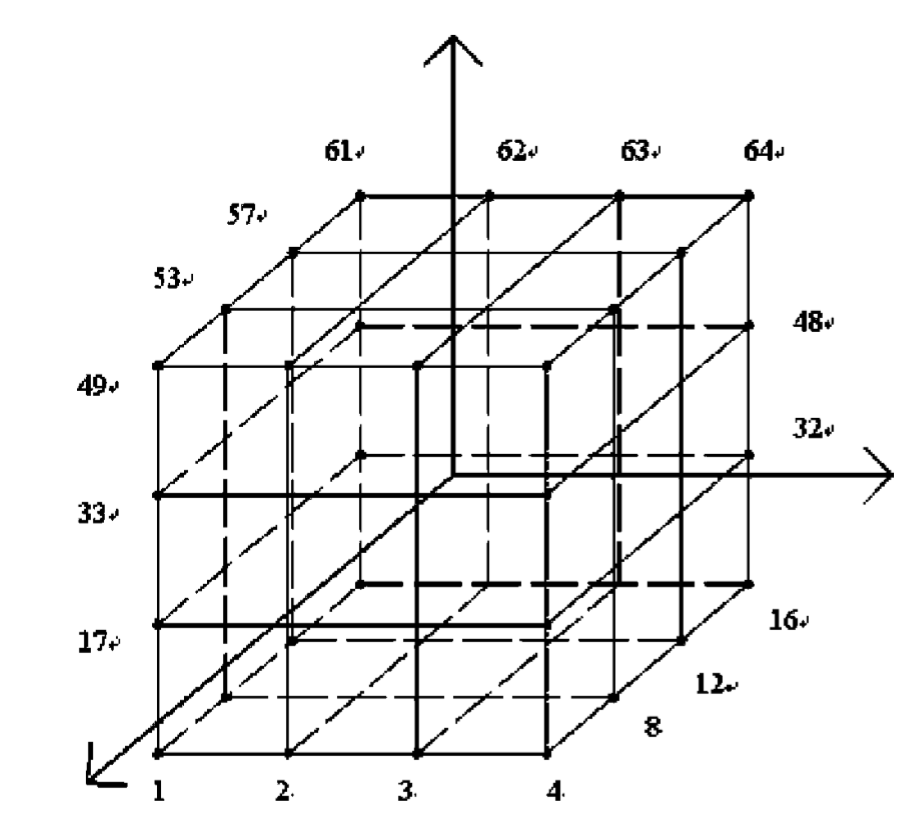
\includegraphics[width=0.75\textwidth]{Logos/VoxelEdges.PNG}
\caption{Darstellung der lokalen 4x4x4 Nachbarschaft  \\ Entnommen aus \protect\cite{hong2003method}} 
\label{fig:nachbarschaft} 
\end{figure}


Ein Gradient ist ein dreidimensionaler Vektor, der in die Richtung der größten Änderung der Intensitätswerte im Volumen zeigt. Ein Beispiel dessen ist in \autoref{fig:gradient} zu sehen. Die Gradienten zeigen von rechts nach links, in die Richtung, in der die Intensitätswerte anwachsen.


\begin{figure}[!h] 
\centering 
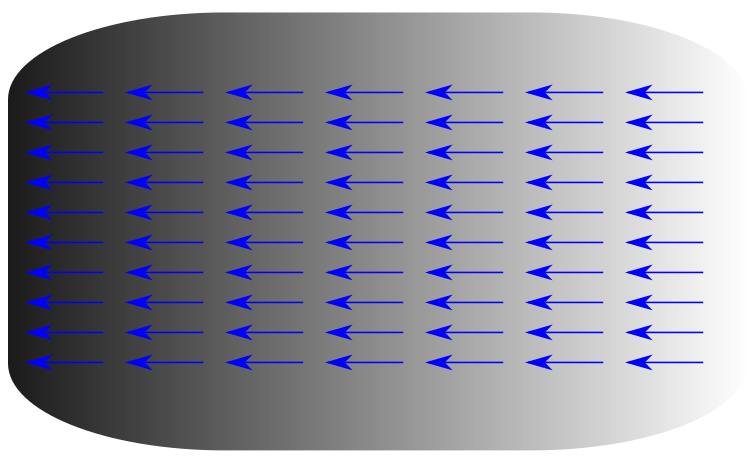
\includegraphics[width=0.75\textwidth]{Logos/Gradient.PNG}
\caption{Beispiel Gradienten} 
\label{fig:gradient} 
\end{figure}



Gäbe es eine Funktion, die die Intensitätswerte des Volumens in der lokalen Nachbarschaft beschreibt, wäre der Gradient die Ableitung dieser Funktion. Folglich muss für die Berechnung eines Gradienten zunächst eine Intensitätsfunktion für die lokale 4x4x4 Nachbarschaft aufgestellt werden. Im Paper wird dies mit der Formel:
\begin{equation}
	f(x,y,z) = Ax^{2}+By^{2}+Cz^{2}+2Fyz+2Gzx+2Hxy+2Ix+2Jy+2Kz+D
\end{equation}
approximiert, da es nicht möglich ist, eine solche Funktion zu bestimmen. Um den Gradienten zu erhalten, muss diese Funktion abgeleitet werden. Für die Berechnung des Gradientenvektor $n$ ergibt sich dadurch die Formel:


\begin{equation}
	n =2\begin{bmatrix}
           Ax + Gz + Hy + I \\
           Hx + By + Fz + J \\
           Gx + Fy + Cz + K
         \end{bmatrix} 
\end{equation}

Um den Gradienten zu berechnen, müssen folglich die Parameter $A$, $B$, $C$, $E$, $F$, $G$, $H$, $I$ ,$J$, $K$ gelöst werden. Dazu wird im Paper zunächst die \textit{error distance} vorgestellt. Diese beschreibt die Entfernung zwischen einem berechneten Datenpunkt und seinem korrespondierenden Punkt in den tatsächlichen Daten. Die Funktion $E$($A$, $B$, $C$, $E$, $F$, $G$, $H$, $I$ ,$J$, $K$) berechnet die Summe der \textit{error distance} aller 64 Nachbarpunkte. Diese Summe drückt aus, wie gut die Approximation die tatsächlichen Intensitätswerte des Volumens beschreibt. Deshalb müssen die Parameter so gewählt werden, dass die Summe $E$ minimal wird und somit die approximierte Intensitätsfunktion das Volumen möglichst genau beschreibt.


\begin{equation}
\begin{array}{l}
  E(A,B,C,D,F,G,H,I,J,K) = \\
	\sum\limits_{k=1}^{64}  w_{k}(Ax^{2}+By^{2}+Cz^{2}+2Fyz+2Gzx+2Hxy+2Ix+2Jy+2Kz+D - f_{k})^2
\end{array}
\end{equation}


Dabei ist $w_{k} = \frac{1}{d_{k}}$, $d_{k} =(x_{k}^2y_{k}^2z_{k}^2)^{1/2}$  die Distanz des k-ten Punktes zum Ursprung des Koordinatensystems, wie es in \autoref{fig:nachbarschaft} zu sehen ist, und $f_{k}$ der Intensitätswert des k-ten Punktes. 
\newline
Die Parameter $A$, $B$, $C$, $E$, $F$, $G$, $H$, $I$ ,$J$, $K$  können mithilfe der Methode der kleinsten Quadrate bestimmt werden. Dies ist ein mathematisches Verfahren, das zu mehreren Punkten eine Funktion bestimmt. Die Funktion beschreibt eine Kurve, bei der die Summe der Abweichung aller Punkte zur Kurve minimal ist. Dies lässt sich auf die Funktion $E$ übertragen. Mithilfe dessen können durch mehrere Umformungsschritte die Parameter berechnet werden. Anschließend kann der Gradient $[X, Y, Z]$ des Punktes $[x, y, z]$ mit folgender Formel, die sich aus der gezeigten Ableitung des Intensitätsfunktion ergibt, kalkuliert werden:


\begin{align}
\begin{bmatrix}
           X \\
           Y \\
           Z
         \end{bmatrix}    
 	= \begin{bmatrix}
           2A & 2H & 2G \\
           2H & 2B & 2F \\
           2G & 2F & 2C
         \end{bmatrix}
         \begin{bmatrix}
           x \\
           y \\
           z
         \end{bmatrix}
	+\begin{bmatrix}
           2I \\
           2J \\
           2K
         \end{bmatrix}
  \end{align}



\subsection{LH-Werte}

Als nächster Schritt folgt die Berechnung der Low- und High-Werte. Diese beschreiben die Grenzen zwischen zwei verschiedenen Materialien. Liegt ein Voxel innerhalb eines Materials, so sind seine LH-Werte gleich. Liegt ein Punkt jedoch an der Grenze zweier Strukturen, so beschreibt der Low-Wert den Intensitätswert des Materials mit dem niedrigeren und der High-Wert das Material mit dem höheren Intensitätswert. Die LH-Werte eines Voxels werden berechnet, indem in die Richtung des Gradienten integriert wird. Hierfür wurde Heun's Methode, eine modifizierte Euler Methode, verwendet. Dies ist ein numerisches Verfahren, um gewöhnliche Differentialgleichungen mit einem Startwert zu lösen. Dabei lautet die für die Integration benutzte Formel:
\begin{equation}
	u_{i+1} = u_{i} + \frac{1}{2}d(\triangledown f (u_{i}) + \triangledown f(u_{i}+d \triangledown f(u_{i}))) 
\end{equation}
Hierbei sind $u_{i}$ und $u_{i+1}$ die Positionen des aktuellen, beziehungsweise des nächsten Voxels. $\triangledown f(x)$ beschreibt den normalisierten Gradienten bei der Berechnung der High-Werte und den normalisierten inversen Gradiente bei der Berechnung der Low-Werte des Punktes $x$ . $d$ steht für die Schrittweite, die in dieser Arbeit auf einen Voxel festgelegt wurde.
\newline
Die Integration stoppt, wenn eine lokale Extremstelle oder ein Wendepunkt erreicht wird. Diese sind daran zu erkennen, dass die Längen der Gradienten an diesen Stellen null sind. Wird ein solcher Punkt erreicht, wird der Intensitätswert des aktuell besuchten Voxels als Ergebnis für den Low- beziehungsweise High-Wert des Startvoxel gespeichert.
\newline
Anschließend wird ein LH-Histogramm mit allen berechneten LH-Wertpaaren erstellt. Hierbei sind auf der x-Achse die Low-Werte und auf der y-Achse die High-Werte angesiedelt. Die Werte der Achsen reichen von null bis zum jeweiligen Maximum der Low- beziehungsweise High-Werte.
\newline
Ein simples Beispiel der LH-Werte ist in \autoref{fig:lh_bsp} zu sehen. Es ist zu erkennen, dass die Voxel innerhalb der Materialien als LH-Werte den Intensitätswert des jeweiligen Materials besitzen. Der Voxel an der Grenze hat als Low- und High-Werte die Intensitäten der beiden Materialien zwischen denen die Grenze verläuft.



\begin{figure}[!h] 
\centering 
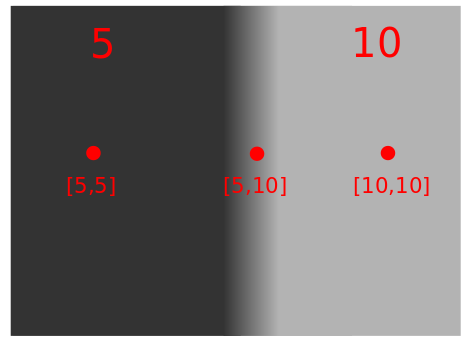
\includegraphics[width=0.75\textwidth]{Logos/LH.PNG}
\caption{Beispiel LH-Werte} 
\label{fig:lh_bsp} 
\end{figure}



\subsection{LH-Clustering}

Als nächstes wird der erste Clusteringschritt durchgeführt. Dieser findet über dem LH-Raum, genauer gesagt auf dem zuvor berechneten LH-Histogramm statt. Dafür wird \textit{Meanshiftclustering} verwendet.
\newline
Vor dem Berechnen der Cluster muss zunächst eine Bandweite sowie ein Thresholdwert bestimmt werden, welche die Sensitivität des Clusterings angeben. Die von Nguyen \cite{nguyen2012clustering} verwendete Bandweite liegt bei 7\% bis 9\% des maximalen LH-Wertes und der Threshold bei 0,01. Anschließend kann die Kalkulation der Cluster beginnen.
\newline
Die Berechnung wird für jeden Punkt im Histogramm durchgeführt. Jede Iteration besitzt dabei einen Cluster mit einen Mittelpunkt. Der Mittelpunkt eines Clusters ist der jeweilige Mittelwert der Low- und High-Werte aller Punkte des Clusters. Wenn die Kalkulation für einen beliebigen Punkt startet, wird dieser zum Cluster hinzugefügt und als erster Mittelpunkt bestimmt. Anschließend werden alle Punkte die im Histogramm in einem Umkreis von der Bandweite um den Mittelpunkt liegen zum Cluster hinzugefügt. Danach wird der neue Mittelpunkt berechnet. Erneut werden alle Punkte, die innerhalb der Bandweite um den Mittelpunkt liegen und noch nicht zum Cluster gehören, hinzugefügt. Dies wiederholt sich so lange, bis die Distanz zweier aufeinanderfolgender Mittelpunkte kleiner als die Bandweite multipliziert mit dem Thresholdwert ist.
\newline
Nachdem diese Berechnung für jeden Punkt im Histogramm durchgeführt wurde, existieren mehrere Cluster, die oftmals aus vielen gleichen Punkten bestehen. Um dies zu unterbinden, werden in einem weiteren Schritt alle Cluster, die sehr nah beieinander liegen, verschmolzen. Dies betrifft jene Cluster, deren Mittelpunkte eine Distanz kleiner als die Hälfte der Bandweite zueinander haben.



\subsection{Räumliches-Clustering}

Anschließend wird der zweite Clusteringschritt durchgeführt, welcher erneut \textit{Meanshiftclustering} verwendet. Dies wird mit dem gleichen Vorgehen, wie im vorherigen Schritt beschrieben, umgesetzt. Ein Unterschied besteht jedoch darin, dass diesmal das Clustering nicht auf dem LH-Raum, sondern auf dem kartesischen Raum des Volumens angewendet wird. Weiterhin wird das Clustering auf den zuvor entstandenen Clustern einzeln und unabhängig voneinander durchgeführt. Dadurch haben alle durch den räumlichen Clusteringschritt entstehende Ergebniscluster ähnliche LH-Werte und liegen auch im Volumen sehr nah beieinander.
\newline
Aus diesem Grund findet am Ende der Berechnung der Cluster keine Verschmelzung statt, da dies den Sinn der beiden von einander getrennten Clusteringschritte zerstören würde. Würden die Ergebniscluster anhand ihrer räumlichen Informationen verschmolzen werden, wäre der erste Clusteringschritt umsonst gewesen, da die Ähnlichkeit der LH-Werte verloren gehen würde.



\subsection{Hierarchisches-Clustering}
 
Im optionalen letzten Clusteringschritt, werden die berechneten Cluster hierarchisch miteinander verschmolzen. Dafür wird zunächst der paarweise Abstand zwischen allen Clustern berechnet. Der Abstand wird wie bei Sereda \cite{sereda2006automating} anhand der Anzahl der direkten Nachbarschaften der Voxel beider Cluster bestimmt. Anschließend werden immer die beiden Cluster, die sich am nächsten sind, zu einem verschmolzen. Dieser Vorgang wiederholt sich so lange, bis nur noch ein Cluster existiert. Im Anschluss wird das Verfahren Schritt für Schritt rückgängig gemacht, bis eine vom Benutzer angegebene Anzahl an Clustern erreicht wird.
\newline
Der vorgestellte dritte hierarchische Clusteringsschritt wurde in dieser Arbeit nicht angewendet. Der Grund dafür ist, dass das Verschmelzen von Clustern abhängig von räumlicher Nähe für die Aufgabe das Ventrikelsystem hervorzuheben nicht zielführend ist. Wird das System als ein oder mehrere Cluster erkannt, liegen diese mitten im Gehirn neben sehr vielen anderen Clustern und würden mit anderen umliegenden Strukturen verschmolzen werden.




















































